Para el orquestrador tendremos las siguientes clases:
\begin{figure}[h!]
    \centering
    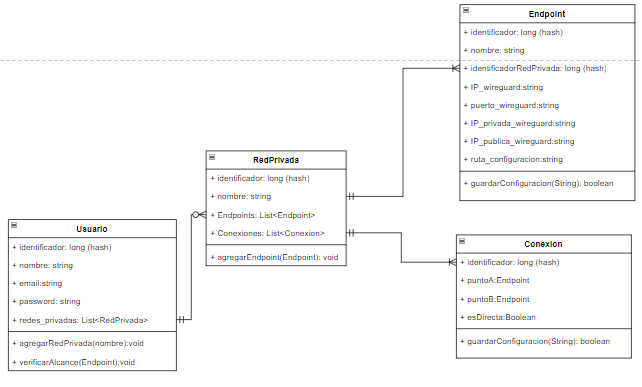
\includegraphics[width=\textwidth]{diagrama-clases.png}
    \caption{Diagrama de clases}
\end{figure}

Bajo la idea de que el orquestrador es el encargado de orquestar la conexión entre los dispositivos finales dentro de una red privada de un cliente, tendremos las siguientes clases:
\begin{itemize}
    \item \textbf{Cliente}: Clase que representa a un cliente que se conecta a la red privada de otro cliente.
    \item \textbf{Endpoiny}: Clase que representa a un dispositivo final que se conecta a la red privada de un cliente.
    \item \textbf{Conexión}: Clase que representa una conexión entre dos dispositivos finales. La idea de esta clase es que el orquestrador sepa que dispositivos finales están conectados entre si y para cuales es necesario relay.
\end{itemize}